\documentclass{dit}

\usepackage{amsmath}
\usepackage{hyperref}
\pdfstringdefDisableCommands{\def\_{_}}
\usepackage{tikz}
% \usepackage{pgfplots}

% allow embedding files in the PDF so viewers can open/save them
\usepackage{attachfile2}

% CSV import for tables
\usepackage{csvsimple}
\usepackage{longtable}
% ensure floats appear before section text when desired
\usepackage{placeins}
% code/listing support for run commands
\usepackage{listings}
\lstset{basicstyle=\ttfamily\small,breaklines=true,columns=fullflexible}

% Macro to show how to run binaries in a consistent way
\newcommand{\runcmd}[1]{\vspace{6pt}\noindent\textbf{Run: }\lstinline!#1!\par}

\usepackage[english,greek]{babel}
% helper to typeset short English fragments when main language is Greek
\newcommand{\en}[1]{\foreignlanguage{english}{#1}}

\newcommand*{\name}{Ευάγγελος Τραϊκόγλου}
\newcommand*{\id}{1115202200189}
\newcommand*{\course}{Παράλληλα Συστήματα}
\newcommand*{\assignment}{Εργασία \en{Openmp}}

\begin{document}

\maketitle

% \tableofcontents
\begin{itemize}
    \item \en{cpu}: \en{i7-8700}
    \item \en{cores}: \en{12 logical, 6 physical}
    \item \en{os, kernel}: \en{Ubuntu 24.04.3 LTS, 6.8.0-87-generic}
    \item \en{comp version}: \en{gcc 13.3.0}
\end{itemize}

\section{\en{Polynomial Multiplication}}
Η πρώτη άσκηση επικεντρώνεται στον πολλαπλασιασμό πολυωνύμων βαθμού \en{n}.
Ο σειριακός αλγόριθμος ακολουθεί την απλή υλοποίηση $\mathcal{O}(n^2)$ χρόνου.
Στον παράλληλο, κάθε νήμα υπολογίζει ένα εύρος του διανύσματος αποτελέσματος σύμφωνα με τον τύπο: 
$res_k = \sum_{i=0}^{k}a_i \cdot b_{k-i}$. Αυτό επιτρέπει τη μη χρήση συγχρονισμού αφού κάθε νήμα
γράφει σε διαφορετικές θέσεις. Η παράλληλη υλοποίηση χρησιμοποιεί την οδηγία (\en{omp parallel for}) για 
τον βρόχο των κ επαναλήψεων και την οδηγία (\en{omp simd reduction(+:sum)}) για την \en{simd} εκτέλεση του
πολλαπλασιασμού στον εσωτερικό βρόχο ($\sim$ 1\en{sec} πιο γρήγορο για αρκούντως μεγάλα πολυώνυμα).
% Example run command for this section
\\
\en{\runcmd{./polynomial_mult -n <degree> -t <threads>}}


% Figures for Polynomial Multiplication
\begin{figure}[htbp]
    \centering
    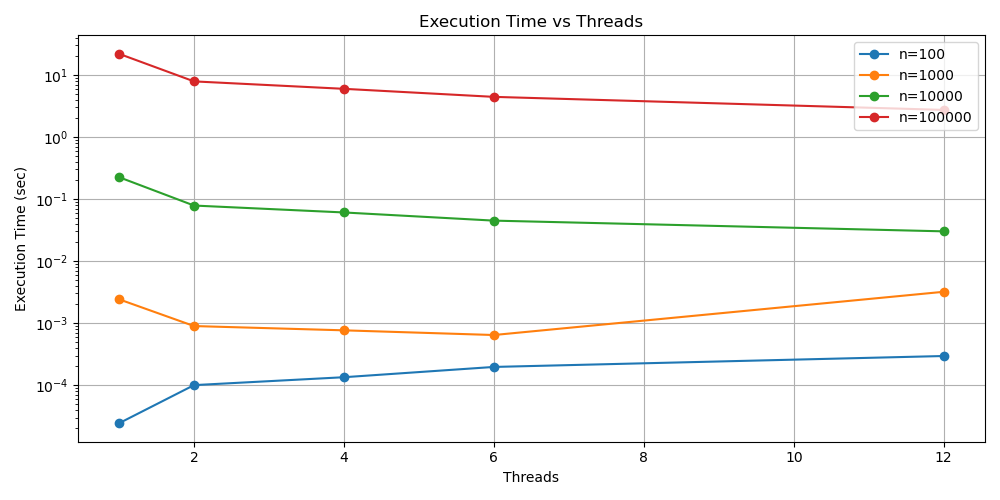
\includegraphics[width=0.8\linewidth]{graphs/execution_time_vs_threads_pol.png}
    \caption{\en{Execution time vs threads for polynomial multiplication}}
    \label{fig:exec_time_vs_threads_pol}
\end{figure}

\begin{figure}[htbp]
    \centering
    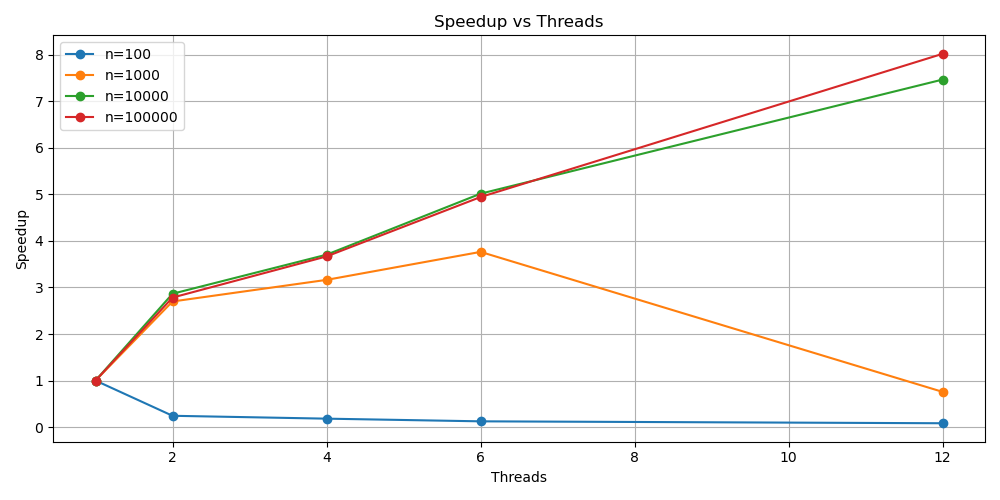
\includegraphics[width=0.8\linewidth]{graphs/speedup_vs_threads_pol.png}
    \caption{\en{Speedup vs threads for polynomial multiplication}}
    \label{fig:speedup_vs_threads_po}
\end{figure}
\FloatBarrier
\underline{Συμπεράσματα}:
Για μικρά \en{n} (πχ 100), η αύξηση των νημάτων αυξάνει τον χρόνο εκτέλεσης αφού επηρεάζεται
κυρίως από την ύπαρξή τους. Κάθως όμως το \en{n} αυξάνεται, η αύξηση των νημάτων επιφέρει μείωση
του χρόνου εκτέλεσης. Βέβαια το κέρδος από την εισαγωγή ενός νέου νήματος μειώνεται, ακολουθώντας
τον νόμο της φθίνουσας απόδοσης. Για \en{n}=1000, παρατηρείται μια απότομη πτώση στην επίδοση πηγαίνοντας
από 6 νήματα σε 12 (όπου λειτουργεί το \en{hyperthreading} πλήρως), πιθανώς λόγω της ανεπαρκούς εργασίας ανά νήμα.
Αντίστοιχα, η επιτάχυνση (με βάση το σειριακό) μεγιστοποιείται στον μέγιστο αριθμό από νήματα (πέραν της
περίπτωσης \en{n}=1000 όπου μεγιστοποιείται για νήματα=6) και για μεγαλύτερες τιμές του \en{n}.

\section{\en{Sparse Matrix-Vector Multiplication}}
Η δεύτερη άσκηση επικεντρώνεται στον αποδοτικό πολλαπλασιασμό πίνακα-διανύσματος με χρήση της
τεχνικής \en{CSR}. Η αρχικοποίηση γίνεται ως εξής:
Κρατούνται τέσσερις πίνακες: \en{values, col\_index, row\_index, row\_nz}.
Ο \en{values} κρατά τις μη μηδενικές τιμές του πίνακα με τη σειρά που διαβάζονται (ανά γραμμές).
Ο \en{col\_index} τις στήλες που αυτές οι τιμές βρίσκονται (με τη σειρά που εμφανίζονται στον \en{values}).
Ο \en{row\_index} πόσα στοιχεία είναι μη μηδενικά πάνω από τη γραμμή \en{i} (πχ \en{row\_index[2]} = πόσα μη
μηδενικά υπάρχουν πάνω από τη γραμμή 2).
Ο \en{row\_nz} πόσα μη μηδενικά υπάρχουν στη γραμμή \en{i}.
Πρώτα αρχικοποιείται ο \en{row\_nz} παράλληλα, μετά ένα νήμα υπολογίζει τον \en{row\_index} πίνακα
(\en{row\_index[i+1] = row\_index[i] + row\_nz[i]}).
Τέλος, αρχικοποιούνται παράλληλα οι \en{values, col\_index}.
Η υλοποίηση του πολλαπλασιασμού είναι ακριβώς όπως περιγράφεται στο: 
\en{\url{https://people.eecs.berkeley.edu/~aydin/csb2009.pdf}}
\\
Δημιουργείται η παράλληλη περιοχή πριν ξεκινήσει ο βρόχος με των \en{iterations} και ένα μόνο
νήμα στο τέλος αντιγράφει το \en{output vector y} στο \en{x} για την επόμενη επανάληψη.
Αν το \en{PAR} έχει οριστεί, τρέχει ο \en{dense parallel} αλγόριθμος αλλιώς ο απλός σειριακός (\en{dense serial, 
default: PAR}).
\\
\en{\runcmd{./sparse -n <matrix size> -p <sparsity:0-100> -i <iterations> -t <threads>}}

\underline{Σημείωση}: 
Όλα τα πειράματα υπάρχουν και στο \en{csv} αρχείο: \en{benchmarks\_sparse.csv}.
Τα παρακάτω διαγράμματα προβάλλουν κάποια αποτελέσματα για δεδομένες τιμές των 
άλλων παραμέτρων (που επιλέχθηκαν για να αναδεικνύουν την υπεροχή του \en{CSR}).

\begin{figure}[htbp]
    \centering
    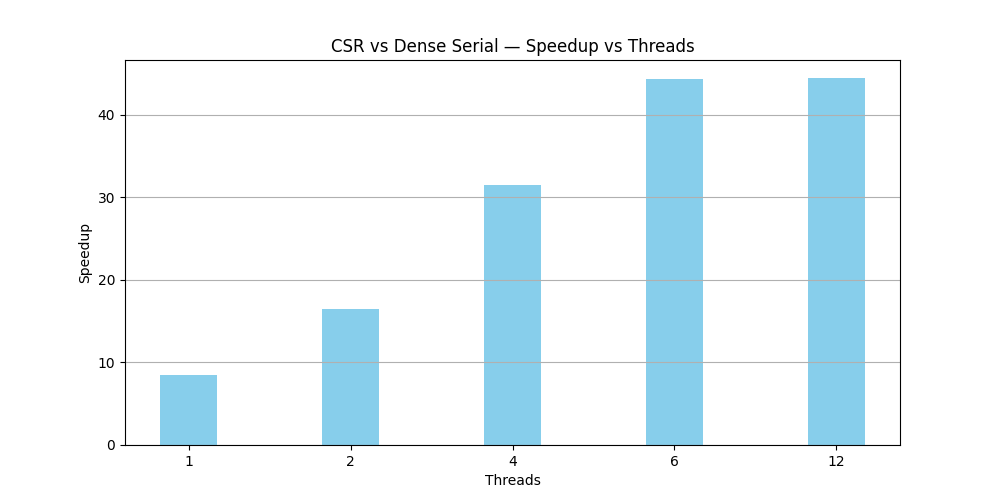
\includegraphics[width=0.8\linewidth]{graphs/speedup_vs_threads_bar_sparse.png}
    \caption{\en{Speedup vs threads: n=10000, sparsity=90, iter=50}}
    \label{fig:sparse_threads}
\end{figure}

\begin{figure}[htbp]
    \centering
    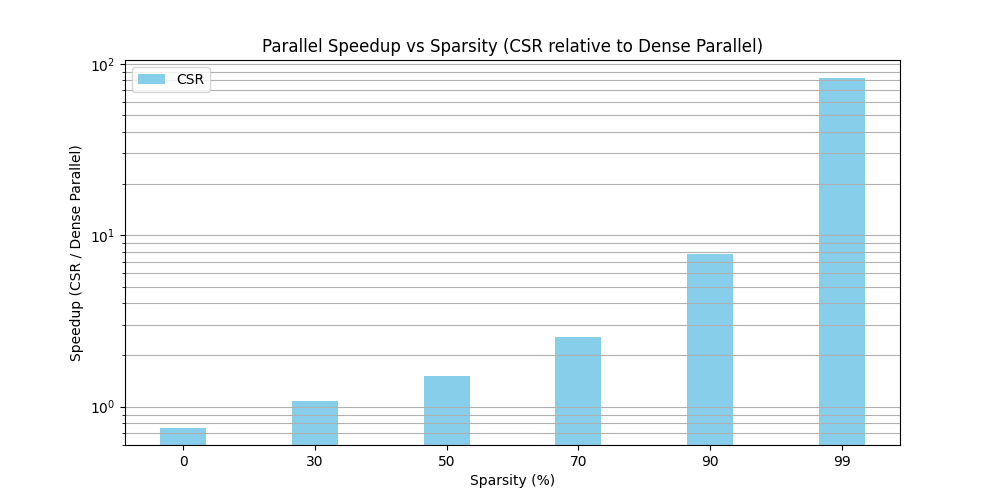
\includegraphics[width=0.8\linewidth]{graphs/speedup_vs_sparsity_bar_sparse.png}
    \caption{\en{Speedup vs sparsity: n=10000, threads=6, iter=50}}
\end{figure}

\begin{figure}[htbp]
    \centering
    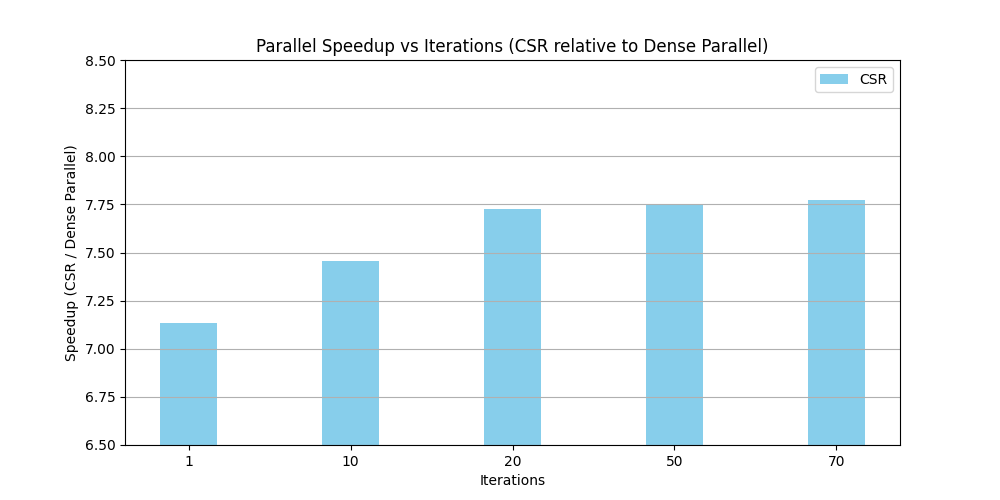
\includegraphics[width=0.8\linewidth]{graphs/speedup_vs_iterations_bar_sparse.png}
    \caption{\en{Speedup vs iterations: n=10000, sparsity=90, threads=6}}
\end{figure}

% comp init with real

\begin{figure}[htbp]
    \centering
    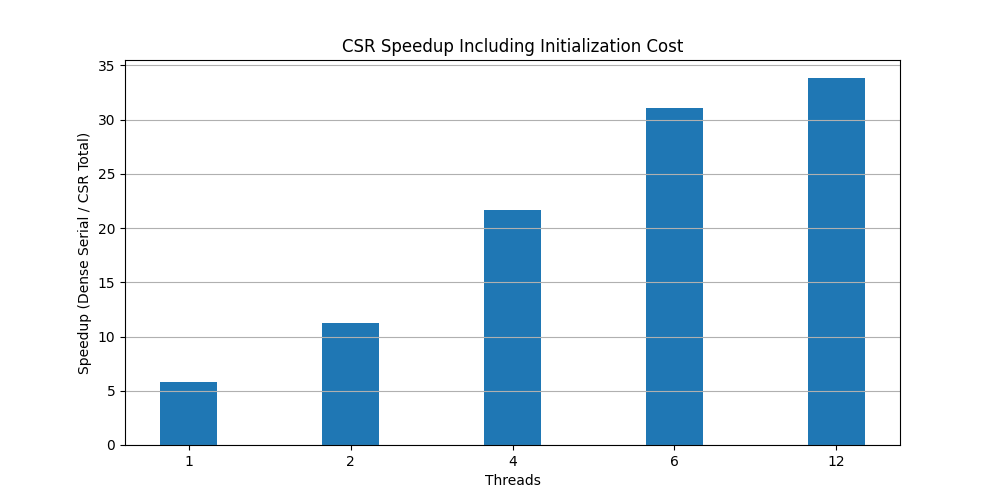
\includegraphics[width=0.8\linewidth]{graphs/speedup_vs_threads_csr_total_bar_sparse.png}
    \caption{\en{Speedup vs threads (Dense serial-CSR total=init+time): n=10000, sparsity=90, threads=6}}
    \label{fig:sparse_csr_total}
\end{figure}

\begin{figure}[htbp]
    \centering
    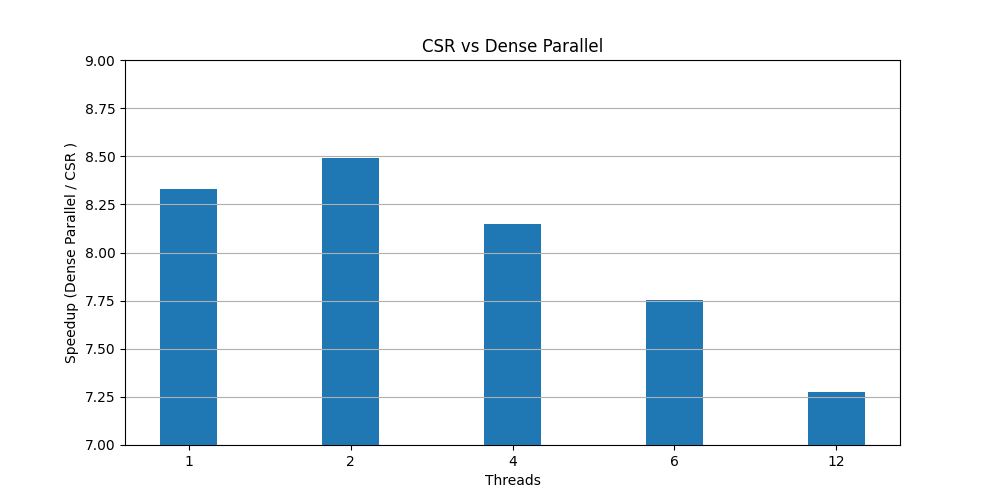
\includegraphics[width=0.8\linewidth]{graphs/speedup_vs_threads_densepar_csr_bar_sparse.png}
    \caption{\en{Speedup vs threads (Dense parallel-CSR): n=10000, sparsity=90, threads=6}}
    \label{fig:sparse_densepar_csr}
\end{figure}

\begin{figure}[htbp]
    \centering
    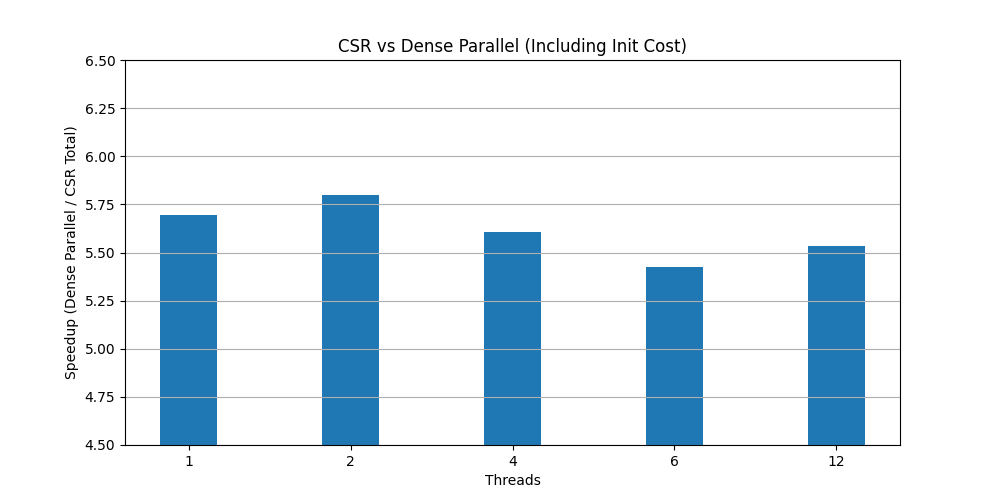
\includegraphics[width=0.8\linewidth]{graphs/speedup_vs_threads_densepar_csrtotal_sparse.png}
    \caption{\en{Speedup vs threads (Dense parallel-CSR total=init+time): n=10000, sparsity=90, threads=6}}
    \label{fig:sparse_densepar_csrtotal}
\end{figure}
\FloatBarrier
\underline{Συμπεράσματα}:
Η επιτάχυνση του \en{CSR} σε σχέση με τον σειριακό αλγόριθμο είναι μεγάλη σε υψηλά \en{sparsity} και
μεγαλύτερους σε μέγεθος πίνακες και προφανώς με την αύξηση των νημάτων γίνεται μεγαλύτερη μέχρι ένα
σημείο. Η μετάβαση από τα 6 νήματα στα 12 δεν δίνει θεμιτή επιτάχυνση ακολουθώντας τον νόμο της 
φθίνουσας απόδοσης. Καθώς αυξάνεται το \en{sparsity} και για αρκούντως μεγάλους πίνακες,
το \en{CSR} υπερτερεί του απλού παράλληλου αλγορίθμου, αφού παραλείπονται οι ανούσιοι πολλαπλασιασμοί.
Επιπλέον, η αύξηση του αριθμού των επαναλήψεων επιφέρει αύξηση στην επιτάχυνση καθώς η υπεροχή του \en{CSR}
δρα αθροιστικά στην αύξηση του πλήθους των επαναλήψεων σε σχέση με την απλή παράλληλη εκδοχή.
Ο χρόνος για την αρχικοποίηση του \en{CSR} αυξάνεται καθώς το πλήθος των μη μηδενικών στοιχείων αυξάνεται
(αφού μεγαλώνουν οι πίνακες \en{values, col\_index, non\_zr}). Άρα η επιτάχυνση του \en{CSR} συνολικά 
(\en{init time + execute time}) είναι μίκροτερη από την σύγκριση με μόνο το \en{execute time}, όπως φαίνεται και
στα αντίστοιχα διαγράμματα (\ref{fig:sparse_threads},\ref{fig:sparse_csr_total},
\ref{fig:sparse_densepar_csr},\ref{fig:sparse_densepar_csrtotal}). 

\section{\en{Mergesort with tasks}}
% Example run command for this section
Η τρίτη άσκηση αφορά την αποδοτική υλοποίηση του \en{mergesort} με τη χρήση των \en{tasks} της \en{Openmp}.
Η σειριακή υλοποίηση είναι η γνωστή. Η παράλληλη δημιουργεί ένα παράλληλο \en{block} πρώτα \en{n} νημάτων
και ένα απο αυτά καλεί την συνάρτηση \en{parallel\_mergesort}. Μέσα στη συνάρτηση τα \en{tasks} δημιουργούνται
αν οι υποπίνακες είναι αρκούντως μεγάλοι ($>$ 20000, οπού η τιμή βρέθηκε μετά από πειράματα). Το νήμα που δημιουργεί
τα \en{tasks} περιμένει να ολοκληρώσουν μέσω της \en{taskwait}.
\\
\en{\runcmd{./mergesort -n <input_size> -c <choice:s,p> -t<threads>}}

\underline{Σημείωση}: 
Τα πειράματα υπάρχουν και στο \en{csv} αρχείο: \en{benchmarks\_mergesort.csv}.

\begin{figure}[htbp]
    \centering
    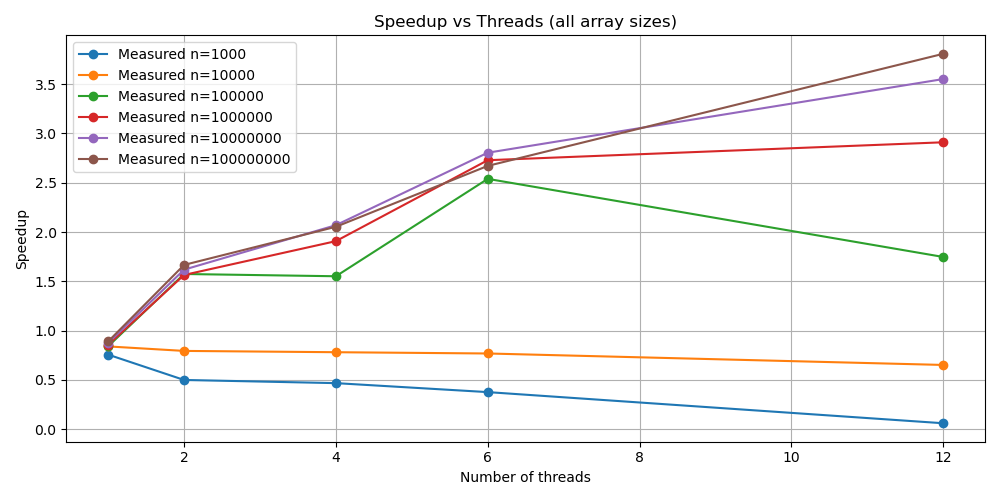
\includegraphics[width=0.8\linewidth]{graphs/speedup_vs_threads_merge.png}
    \caption{\en{Speedup vs threads for mergesort}}
\end{figure}
\FloatBarrier
\underline{Συμπεράσματα}:
Η επιτάχυνση που παρατηρείται σε σχέση με τη σειριακή υλοποίηση είναι περιορισμένη.
Αφενός λόγω της σειριακής εκτέλεσης του \en{merge} βήματος, το οποίο χρειάζεται να
αντιγράψει στους δύο καινούργιους υποπίνακες ένα εύρος στοιχείων του αρχικού πίνακα
και αντίστοιχα να τους αποδεσμεύσει (αν έχουν δεσμευθεί με \en{malloc}). Ο αλγόριθμος
δηλαδή είναι \en{memory-bound}, για αυτό δεν πετυχαίνεται καλή επιτάχυνση. Σε κάποιες
περιπτώσεις, η μετάβαση από τα 6 στα 12 νήματα επιφέρει επιβράδυνση, κυρίως στα μικρότερα
μεγέθη πινάκων.



\end{document}